\documentclass[sigconf]{acmart}

% remove copyright footer
\setcopyright{none}
\settopmatter{printacmref=false}
\renewcommand\footnotetextcopyrightpermission[1]{}

\fancyhf{}

% encoding and language
%\usepackage[english]{babel}
\usepackage[T1]{fontenc}
\usepackage[utf8]{inputenc}

\usepackage{booktabs}
\usepackage{balance}
\usepackage[caption=false]{subfig}
\usepackage[toc,acronym,shortcuts]{glossaries}
\usepackage{hyperref}

\def\pprw{8.5in}
\def\pprh{11in}
\special{papersize=\pprw,\pprh}
\setlength{\paperwidth}{\pprw}
\setlength{\paperheight}{\pprh}
\setlength{\pdfpagewidth}{\pprw}
\setlength{\pdfpageheight}{\pprh}

\newacronym{IoT}{IoT}{Internet of Things}

\usepackage{xspace}
\newcommand{\scapy}{Scapy\xspace}

\begin{document}

\title{Security for the Internet of Things - CoAP Fuzzing}

\author{Jan Ehmueller and Justin Trautmann \\ \today}

\begin{abstract}
\begin{enumerate}
	\item Mit wenigen Worten das Problem einführen
	\item Wichtigste verwandte Arbeit erwähnen
	\item Eure wissenschaftlichen Beiträge umreißen
	\item Zusammenfassung der Ergebnisse
\end{enumerate}
\end{abstract}

\maketitle

\glsresetall

\section{Introduction}
\label{section:introduction}

%\begin{enumerate}
%	\item Kontext einführen
%	\item Problem darstellen
%	\item Den diesbezüglichen Stand der Technik zusammenfassen
%	\item Eure wissenschaftlichen Beiträge auflisten
%\end{enumerate}

Nowadays, already 8.4 billion connected things are part of the Internet of Things (IoT)~\cite{IoTForecastGartner} and it is constantly growing so that a number of around 30 billion devices can be expected by the year 2020~\cite{IoTForecastNordrum}. IoT devices are used in a variety of application scenarios but have in common, that they are usually heavily constrained with respect to the computation power due to battery restrictions and size. Nonetheless they are mostly connected to the internet and can be accessed from anywhere. Since IoT systems often involve highly personal or enterprise data and mechanisms, this leads to a high demand for security. 

In constrained environments, the conventional internet protocol stack can be hardly applied. Therefore most IoT devices run a protocol stack composed of especially designed low-power protocols for constrained environments. One such commonly used stack is composed of IPv6 over Low-Power Wireless Personal Area Networks (6LoWPAN), a low-power adaption of wireless IPv6, IPv6 Routing Protocol for Low-Power and Lossy Networks (RPL), a routing protocol for low-power and lossy networks and Constrained Application Protocol (CoAP), an application level protocol for constrained devices based on UDP. CoAP is not limited to run on these specific underlying protocols but since Contiki-NG uses this protocol stack, other protocol combinations will not be considered. Though all of the protocols can become potential attack vectors, we will subsequently focus on CoAP. 

CoAP was designed in order to enable constrained devices to perform internet communication without the need to perform high-overhead HTTP communication. Its simplicity and the multicast ability make CoAP very suitable for IoT networks.
CoAP is known to be possibly vulnerable with respect to protocol parsing, URI processing, proxying and caching, risk of amplification, IP address spoofing and many more. Since some of these vulnerabilities are due to the underlying UDP, protocol parsing and URI processing are especially interesting when assessing CoAP security. Additionally to the inherent vulnerabilities of CoAP, the Contiki-NG implementation suffers from additional vulnerabilities. Low-level C implementations tend to cause unexpected memory leaks and the lack of additional security mechanisms such as AddressSanitizer make it hard to detect them a priori.

Finding vulnerabilities in a software systems in conjunction with a hardware system is always a hard task and many methods such as manual testing or code review can only focus on one aspect of the system. Therefore fuzzing can help to find surprising vulnerabilities even in a black-box setting. It can be fully automated, run a security analysis with no runtime overhead and no or only little explicit expert knowledge about the system under test is needed.

Our approach consists of an automatic setup phase of the IoT devices and the fuzzer and the actual fuzzing with logging of all send and received messages and debug output of the systems under test. A CoAP message is crafted using a CoAP message template and informed random field values. Subsequently, the message is send to a IoT border router that routes it to a IoT CoAP server. If needed, a response is transferred back and the request as well as the response are written to log files. Furthermore, all debug outputs of the border router and the CoAP server are saved as well. In order to check if fuzzing was successful and a crash occurred, a request to the standardized CoAP route \textit{/.well-known/core} that returns all available routes is performed and the response is compared to the expected value. If a variation or even no response can be detected, the fuzzing has been successful. The whole fuzzing workflow is automatically repeated until interrupted by the user.

To the best of our knowledge, there is little to no work on CoAP fuzzing on real IoT devices. Melo et al.~\cite{Melo2017RobustnessTO} targeted only CoAP implementations with no respect to the underlying hardware and Chen et al.~\cite{chen2018ndss} focused on indirect CoAP fuzzing by using the smartphone apps of specific IoT devices. Therefore fuzzing a conjoined system of any embedded hardware and a CoAP implementation seems promising for finding further unknown vulnerabilities. Also Muench et al.~\cite{EURECOM+5417} elaborated on different approaches to evaluate fuzzing and detect corrupted behavior aside from total device failures.
\section{Background}
\label{section:background}

%\begin{enumerate}
%	\item Relevante Protokolle und Konzepte einführen
%	\item Auf das beschränken, was zum Verstehen der nachfolgenden Abschnitte notwendig ist
%	\item Bei Platzmangel könnt ihr diesen Abschnitt auch weglassen und stattdessen bei den entsprechenden Stellen Verweise einfügen
%\end{enumerate}

\subsection{CoAP}

The CoAP protocol defined in RFC7252 a lightweight and RESTful protocoll that can be easily mapped on HTTP~\cite{RFC7252}. Basically, four types of messages can be transferred via UDP. A request can consist of Confirmable (CON) and Non-confirmable (NON) messages. Confirmable messages are expected to be responded by an Acknowledgment (ACK) message. Furthermore, reset messages (RST) can be send. Non-confirmable messages don't require any response but a response can be send as a NON message. All of these message types can use the four methods GET, PUT, POST and DELETE and get back defined status codes that are very similar to their corresponding HTTP methods and codes. Furthermore, every message is identified by an ID and a token and can be adjusted by several options. In \Autoref{section:approach} we further describe and evaluate specific properties of the CoAP message fields.

\subsection{Hardware}

Our target system for the security evaluation was an OpenMote Rev. A1\footnote{\url{www.openmote.com}} which mainly consists of a CC2538 SoC\footnote{\url{www.ti.com/product/CC2538}} running Contiki-NG~\cite{contiki}. As CoAP server implementation target, the Contiki-NG example implementation\footnote{\url{https://github.com/contiki-ng/contiki-ng/blob/develop/examples/coap/coap-example-server/coap-example-server.c}} was used.

\subsection{Fuzzing}

On the attacker side, we used the python packet manipulation framework \scapy\footnote{\url{https://scapy.net}} with its latest CoAP community contribution\footnote{\url{https://github.com/secdev/scapy/blob/master/scapy/contrib/coap.py}}. This enables us to easily assemble CoAP messages, perform requests and log the responses.

Fuzzing techniques can be categorized with respect to the approach into random fuzzing, mutational fuzzing and generational fuzzing and with respect to the target system into white-box, gray-box and black-box fuzzing~\cite{neystadtPenTesting}.
Random fuzzing is the most inefficient technique with respect to the potentially found errors but relatively simple to set up and best suited for systems that are completely unknown (black-box fuzzing). If some details about the used protocol or message format are known, random fuzzing can be adapted to informed fuzzing so that specific fields such as checksums are still valid in order to avoid instant rejection of the messages.
Mutational fuzzing is based on previously captured valid communication with the system under test that is altered in order to get potentially malicious messages. These messages are still very similar to the usual messages and thus they are not immediately rejected by security mechanisms, which causes them to have a high chance to cause damage.
Lastly generational fuzzing is based on the known structure of the protocol and therefore not suited for black-box fuzzing. Using an empty skeleton of a valid message, fields are randomly or informed randomly filled with values. This makes sure that the message can at least be parsed by the system under test and mechanisms, which are deeper than only the message parser, can be reached and tested.

\section{Related Work}
\label{section:related_work}

% \begin{enumerate}
% 	\item Umfänglichere Diskussion verwandter Arbeiten
% 	\item Vergleichend mit eurem Ansatz
% 	\item Manchmal bietet es sich an diesen Abschnitt erst vor den Conclusions zu bringen
% \end{enumerate}

Previous work on CoAP fuzzing is sparse and only focused on implementation fuzzing. Melo et al.~\cite{Melo2017RobustnessTO} searched for publicly available CoAP implementations on common repository services and search engines and selected a few for testing. Their testing system consisted of the boofuzz framework\footnote{\url{https://github.com/jtpereyda/boofuzz}} in order to start, stop and monitor the systems under test and several \scapy based fuzzing engines. They applied random, mutational and generational fuzzing. As expected, generational fuzzing caused way more crashes than informed random and random fuzzing.

Chen et al.~\cite{chen2018ndss} based their work on the observation that the firmware of most commercial IoT devices is not publicly available but often official smartphone apps are used to communicate with the device. Therefore the app can be used to generate more sophisticated fuzzed messages than random fuzzing would do. They put 17 systems under test that also run different protocols than CoAP and found 8 previously unknown failures.

Furthermore Muench et al.~\cite{EURECOM+5417} addressed the problem of error detection while fuzzing embedded devices in general. Usually total system crashes are used as indicators for successful fuzzing. Unfortunately a variety of software failures such as bugs that cause unintended branching and bring the program in an invalid state or buffer overflows that cause memory corruption and potential execution of data don't cause immediate crashes but lead to general malfunction of the system or cause a crash way later in time. These types of failures are especially hard to find on embedded devices because there are usually just a few mechanisms for memory isolation and protection in place. The authors propose several techniques in order to find these failures even on embedded devices. This includes static instrumentation of the source code or the compiled binary itself with additional memory protection mechanisms, running the software on a more sophisticated host and employ higher level security mechanisms or emulate the device fully or partially. Also hardware instrumentation via debug ports is discussed but rarely applicable on commercial products. Furthermore, different heuristics in order to detect memory corruptions are presented.

Tools for automated code instrumentation in order to detect memory corruptions like the AddressSanitizer~\cite{addressSanitizer} can reliably find memory corruptions when using allocators for memory access. Unfortunately Contiki-NGs memory access is mainly based on global static buffers and therefore cannot be tracked with custom allocators.

Other approaches on fuzzing different layers of the IoT network stack have been made by Böning et al.~\cite{PawelLeo} who targeted the Contiki-NG RPL implementation on fully emulated devices.

Different to all previous approaches, we tried to apply multiple fuzzing methods on a CoAP implementation running on a real IoT device in order to find software errors as well as hardware related errors, which may be impossible to find in an emulator.

\section{Approach}
\label{section:approach}

\begin{enumerate}
	\item Präsentation eures Ansatzes
	\item Meistens bietet es sich an erst die grobe Idee zu vermitteln und dann erst ins Detail zu gehen
	\item Auf interessante und wichtige Design-Entscheidungen eingehen
	\item Modelle einsetzen
\end{enumerate}

Since we intend to fuzz a CoAP implementation running on a real IoT device we needed to decide on a setup that enables us to properly send messages with a high throughput and to implement a fuzzer in an easy-to-use high-level language. Having these goals we decided against fuzzing as an internal attacker from an embedded device in the IoT network, since it has limited resources compared to a desktop or laptop. It would also mean that we would need to implement the fuzzer in C, which would take us longer and it would be harder to implement features compared to a scripting language like python.

We therefore decided to fuzz the IoT device as an external attacker from a laptop that is not part of the IoT network. To do so we need to be able to communicate with the embedded device via IPv6, which is possible if we set up one OpenMote as a border router and a second one as a CoAP server. Via the border router we can send messages via IPv6 into the IoT network and therefore send messages to the CoAP server. The CoAP server uses the Contiki-NG CoAP implementation and runs its CoAP example server on the application layer. Since we only want to fuzz CoAP it does not matter to us what the server on the application layer does with the payload of the CoAP messages.

Having decided on the setup we chose to implement the fuzzer in python and similarly to Melo et al.~\cite{Melo2017RobustnessTO} we use \scapy to create crafted CoAP packets and send them to the IoT device. Our fuzzing workflow looks as follows. We first send a crafted packet to the CoAP server and await a possible response. After getting the response or getting a timeout (e.g., after sending a NON-message) we then test if the IoT device is still reachable or if it somehow does not respond to messages anymore (e.g., due to a crash or some other malfunction). 

\begin{figure}[h]
		\centering
		TODO
		% \includegraphics[width=0.5\textwidth]{img/coap_header}
		\caption{CoAP header fields defined in the CoAP RFC~\cite{RFC7252}}
		\label{figure:coap_header}
\end{figure}

After determining the message flow we now needed to decide how the craft the CoAP packets. We first read the CoAP RFC and analyzed the CoAP message header in \Autoref{figure:coap_header}. Since we know the protocol being used we chose generational fuzzing as fuzzing approach. And as Contiki-NG is open source we can verify how the header fields are handled and parsed which allows to employ white-box fuzzing. We further describe how we fuzz each header field:
\begin{enumerate}
	\item \textbf{Version}: there is currently only one version of CoAP so the version has to be always 1. Contiki-NG has a simple equality check for this field so there is no point in fuzzing this field.
	\item \textbf{Message Type}: since all four message types are valid we simply randomly fuzz this field.
	\item \textbf{Token Length}: this field contains the length of the token field, which is needed because CoAP has a lot of implicit field sizes in its header. The lengths 9 to 15 are reserved according to the RFC and Contiki-NG tests whether this field is larger than 8~\cite{RFC7252}. We therefore fuzz this field randomly in the range [0, 8].
	\item \textbf{Status Code}: every not implemented status code is simply caught by the implementation. Therefore, we randomly choose either a request or a response status code.
	\item \textbf{Message ID}: this id identifies CoAP messages for the purposed of deduplication and response matching. It has a random value anyway, which means that we do not gain anything by fuzzing this field. But we still need to set it randomly to be able to properly send and receive our crafted CoAP messages.
	\item \textbf{Token}: this field is practically the request id. The length of this field can differ from the token length field, since there are no well-defined boundaries for the following fields. That means it can not be checked if the token is too long or too short. We set this value randomly, but the byte length is independent from the value of the token length field.
	\item \textbf{Options}: CoAP options are parsed by reading the bytes after the token and trying to parse them as an option. These options each have small headers themselves, but unfortunately \scapy does enable us to fuzz these option headers as well.

	After an option was successfully parsed, the next byte is looked at and if it is not the payload marker, the following bytes are parsed as options as well. This goes on until a payload marker is found, which then means that after it, a payload with a non-zero lengths follows.

	We fuzz the CoAP options by randomly selecting a number of options implemented by Contiki-NG, which implements a few more options than those defined in the RFC~\cite{RFC7252}. The values for these options are random strings with a length of 0 to 12.
	\item \textbf{Payload}: the payload goes from the first byte after the payload marker to the last byte of the UDP datagram. Since the payload is not touched by the CoAP engine of Contiki-NG we do not fuzz it.
\end{enumerate}

The final decision we now have to make is how we want to detect if the IoT device crashed or malfunctioned after we sent it a crafted CoAP packet. We discussed the following approaches:
\begin{enumerate}
	\item \textbf{Pinging the device}: the simplest approach to test if a device is still reachable in a network is to ping it. This also works with our IoT devices but since an ICMP echo request is handled on the IP layer, it does not reach the CoAP layer and might be answered even though the CoAP engine somehow malfunctioned.
	\item \textbf{Well-known-core request}: according to the RFC, every CoAP server needs to implement the URI-route ``/.well-known/core``, which describes the resources provided by the server~\cite{RFC7252}. This basically acts as a CoAP ping for us, since it is a route every CoAP server has to provide and to respond to the request the CoAP engine is used. If the content of the response is known, the response after each fuzzing request can be tested for proper structure as well, i.e., that the returned content was not somehow changed by the CoAP engine malfunctioning.
	\item \textbf{Filter CLI output of CoAP server}: we can filter the standard output of the CoAP server for error messages and the log messages of the hardware watchdog, that restarts the device if it froze (e.g., in an infinite loop). We can then add timestamps to the whole standard output and match those with timestamps of the fuzzing requests.
	\item \textbf{Add logging to Contiki-NG}: since Contiki-NG is open source, it is possible to simply add more log output to the CoAP implementation to test, for example, memory content of the global buffers used by Contiki-NG.
	\item \textbf{JTAG debugging}: it is possible to attach a debugger via JTAG to the OpenMotes and read out all the memory. This also enables testing of the validity of the memory and to detect writing into sections of memory that should not be written to by the CoAP implementation.
\end{enumerate}

We decided to test the availability of the IoT device via the Well-known-core request, since it is the most straightforward way to check the reachability of the OpenMote and to check that the CoAP implementation still works.

\section{Implementation}
\label{section:implementation}

%\begin{enumerate}
%	\item Überlick über eure Implementierung
%	\item Modell der Softwarearchitektur
%\end{enumerate}

We first implemented a script to fuzz a CoAP server. The workflow of that script is shown in \Autoref{figure:fuzz_flow_chart}. As we described in \Autoref{section:background}, we use \scapy and its CoAP community contribution\footnote{\url{https://github.com/secdev/scapy/blob/master/scapy/contrib/coap.py}} to create crafted CoAP packets. We test the availability of the IoT device after each crafted packet by sending a CoAP request to the URI ``/.well-known/core`` as we reported in \Autoref{section:approach}. We log the timestamp, the fuzzed request, its response and the result of the ``well-known-core`` check for each crafted packet.

\begin{figure*}
	\centering
	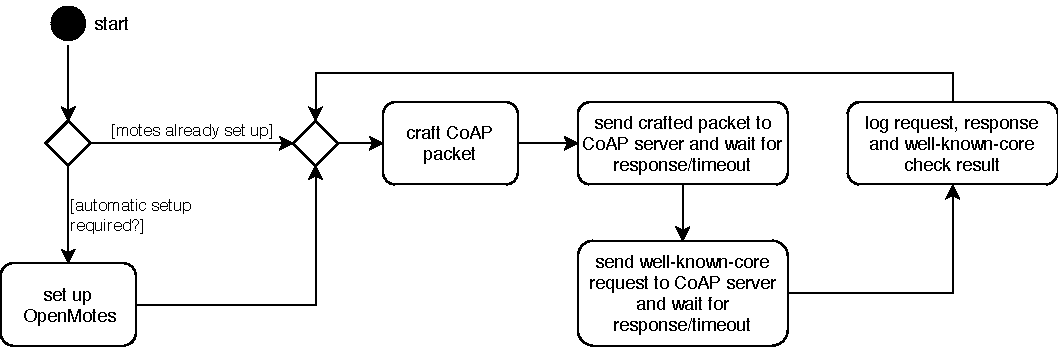
\includegraphics[width=\textwidth]{images/fuzzing_flow_chart}
	\caption{Flow chart of the fuzzing script}
	\label{figure:fuzz_flow_chart}
\end{figure*}

The CoAP implementation of Contiki-NG actually not only implements the CoAP RFC but it also implements extension RFCs, like the Block-Wise Transfers RFC\footnote{\url{https://tools.ietf.org/html/rfc7959}}. This means that the first response to the ``well-known-core``request contains only the first 64 bytes of the response and an option that more packets follow. But the CoAP community contribution of \scapy does not implement any extension RFCs of CoAP and therefore it does not support the Block-Wise Transfer RFC. This results in us only being able to test the first 64 bytes of the response to the ``well-known-core`` request unless we implement the Block-Wise Transfers RFC ourselves. But for our purposes it's enough to simply compare the first 64 bytes of the response.

We also implemented a second script that is able to replay a request that we logged in our first script and it then displays the response and the result of the ``well-known-core`` check. We created this script to test the reproducibility of a request that resulted in a device malfunction. We also added a simple error to the CoAP implementation of Contiki-NG to test if we were able to find such an error. This error caused the hardware watchdog to restart the CoAP server. We were indeed able to find this error.

For convenience we also created bash scripts to automatize the setup of the OpenMotes with the border router and the CoAP server. This enables us to start fuzzing by simply connecting the two OpenMotes to our computer and then just running a single command, which is our python script.

\section{Evaluation}

\begin{enumerate}
	\item Evaluierung interessanter Aspekte anhand von Statistiken
\end{enumerate}

When performing fully automated fuzzing, processing of one fuzzed message takes around 5.2 seconds. Setup times for the devices can vary due to cached binaries but can reach the magnitude of several minutes. In order to evaluate the fuzzer and the system under test, we performed 20.000 runs but did not succeeded to trigger a crash. Nonetheless we ensured that potential crashes can be found by our setup by intentionally adding an infinite loop to the CoAP server implementation as reaction to a specific message.  

The scapy tool turned out to be easily usable in order to automatically construct CoAP messages. Even though a random fuzz method is also available in scapy, we decided to fuzz the message fields by ourselves in order to perform informed random or generational fuzzing. Unfortunately, scapy doesn't implement further very common CoAP RFCs. So the observation of CoAP resources like proposed in RFC7641 and the block-wise transfer of larger messages as proposed in RFC7959 is not implemented. Since the system under test does implement these RFCs, this would be a starting point for further research and could be done by either augmenting the scapy CoAP contribution or the fuzzer itself. This also leads to upper bounds with respect to the message size, because CoAP messages should not exceed a IPv6 MTU in order to avoid fragmentation. 


\section{Conclusions and Future Work}
\label{section:conclusion}

%\begin{enumerate}
%	\item nochmal auf das Ursprungsproblem und dessen Relevanz zurückkommen
%	\item nochmal zusammenfassen was ihr beigetragen habt
%	\item Schlussfolgerungen ziehen
%	\item Vorschläge für zukünftige Forschungsrichtungen
%\end{enumerate}

With the goal of building a fully automated fuzzing system for the CoAP implementation of Contiki-NG, we analyzed the implementation and the CoAP protocol itself in order to employ generational fuzzing. With our setup using the Pyhon framework \scapy and the OpenMote hardware, we performed extensive fuzzing but did not succeed to find serious vulnerabilities in the implementation. This should not be seen as a proof of security and treated carefully since fuzzing can never exhaustively test all possible inputs. Nonetheless it is an indicator for a sufficiently secure implementation.

\scapy turned out to be easily usable in order to automatically construct CoAP messages. Even though a random fuzz method is also available in \scapy, we decided to fuzz the message fields by ourselves. This enables us to perform informed random and generational fuzzing. Unfortunately, \scapy does not implement further CoAP extension RFCs. Such RFCs are the observation of CoAP resources proposed in RFC7641\footnote{\url{https://tools.ietf.org/html/rfc7641}} and block-wise transfers of larger messages proposed in RFC7959\footnote{\url{https://tools.ietf.org/html/rfc7959}}. Since the system under test does implement these RFCs, this would be a starting point for further research and could be done by either extending the \scapy CoAP contribution or the fuzzer itself. The lack of block-wise transfer also leads to upper bounds with respect to the message size, because a single CoAP message should not exceed an IPv6 MTU in order to avoid fragmentation.

Furthermore, different improvements of the fuzzer can be considered in future. For example, lots of IoT devices use the payload message format CBOR\footnote{https://tools.ietf.org/html/rfc7049} that can be fuzzed as well. Doing so would enable the fuzzer to not only find vulnerabilities in the protocol parsing and handling but also in the payload processing logic. 

Also the logging and replay could be improved by providing a feature for selective display of particular messages or errors and more usable replay. In case of a detected error, automatic replay could be considered.

Since the error detection currently relies on the pure observation of the devices output, some errors might have happened but could not be detected by our system. Such errors include any kind of memory corruption that can potentially lead to malfunctioning in the future but cannot be detected from the outside at the moment of occurrence. In order to detect them immediately, the implementation or the device has to be additionally instrumented, which makes the fuzzer no longer generic to all devices and implementations but could be considered too.


% visually balance both columns
\balance

\bibliographystyle{ACM-Reference-Format}
\bibliography{bibliography}

\end{document}
